\section{Explicación del Proyecto}

El proyecto consiste en el diseño y desarrollo de un generador de señal senoidal utilizando un PIC18F45K50, con el objetivo de generar frecuencias de 125 Hz, 250 Hz y 500 Hz, que son mostradas en un display de 7 segmentos. Se implementa un sistema de muestreo y control mediante un Timer 0 que permite la producción de la señal a través de un DAC, y la interacción del usuario se realiza mediante un teclado, que valida y actualiza la frecuencia seleccionada, proporcionando confirmaciones auditivas. Además, el dispositivo envía y recibe datos a través de comunicación serial USART, respondiendo a consultas sobre la frecuencia y actualizaciones de comandos, asegurando una experiencia interactiva y eficiente. Se espera entregar un informe que detalle el desarrollo del proyecto, incluyendo diagramas de flujo y cálculos necesarios, junto con el código fuente en un archivo .zip.

\section{Cálculos para generar las bases de tiempo}

Los calculos para la configuración del tiempo(Timer 0) fueron los siguientes, con el modo de 16 bits($T08BIT = 0$):

\begin{equation*}
    T = \frac{4}{F_{osc}} \ast (PRESCALER) \ast(65355-TMR0)
\end{equation*}

Se uso un tiempo de $4\si{\milli\second}$, lo que el Timer0 será: 

\begin{equation*}
    TMR0 = 53355
\end{equation*}

Se usa entonces: $tm0h = 0xd1$ y $tm0l = 0x1f$. Para el espaciado entre muestras también se puede usar un \textbf{delay us()}, con los valores de $62.5\si{\milli\second}$($500\si{\Hz}$), $125\si{\milli\second}$($250\si{\Hz}$) y $250\si{\milli\second}$($125\si{\Hz}$).

\section{Valores usados para la configuración del DAC}

Los valores usados para el DAC fueron los siguientes:

\begin{verbatim}
    //Configuración del DAC
    
    VREFCON1bits.DACEN = 1;     //HABILITO EL DAC
    VREFCON1bits.DACLPS = 1;    //FUENTE DE TENSION DE BAJA POTENCIA A Referencia positiva
    VREFCON1bits.DACOE = 1;     //HABILITO TENSION DE SALIDA DEL DAC
    VREFCON1bits.DACPSS = 0b10; //FUENTE POSITIVA DEL DAC
    VREFCON1bits.DACNSS = 0;    //FUENTE NEGATIVA DEL DAC a VSS
    VREFCON2bits.DACR = 0b1111; //Bits de selección de salida de voltaje DAC
    VREFCON0bits.FVREN = 1;     //Habilito el valor de referencia ajustado
    VREFCON0bits.FVRS = 0b11;   //FVRS con 4.096 Volts
    VREFCON0bits.FVRST = 1;     //Salida de voltaje ajustado listo para usar
\end{verbatim}

\section{Diagramas de flujo} 

\subsection{Main}

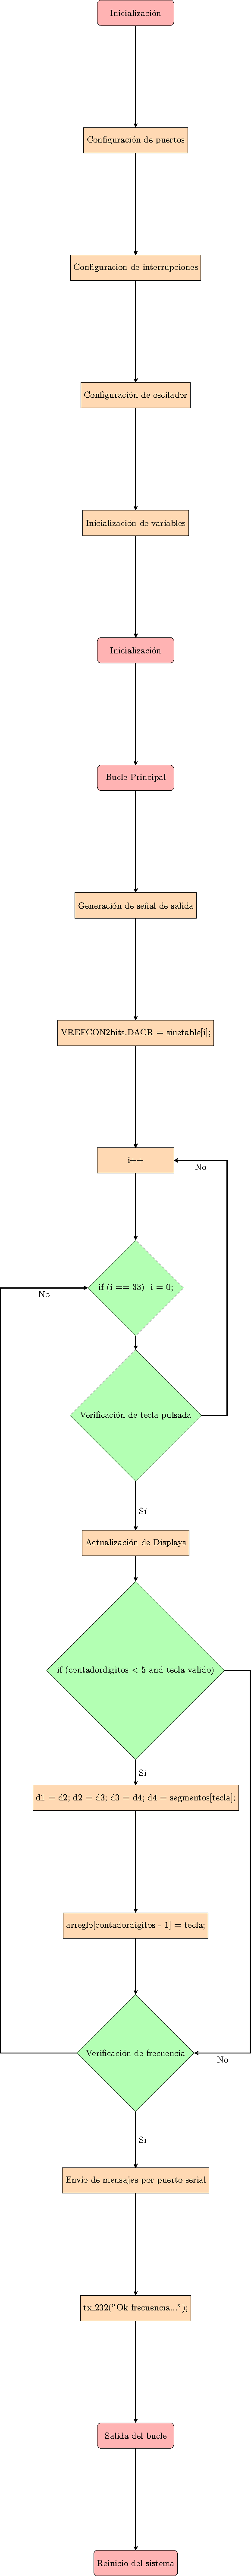
\includepdf{fmain.pdf}

\subsection{Interrupcion}
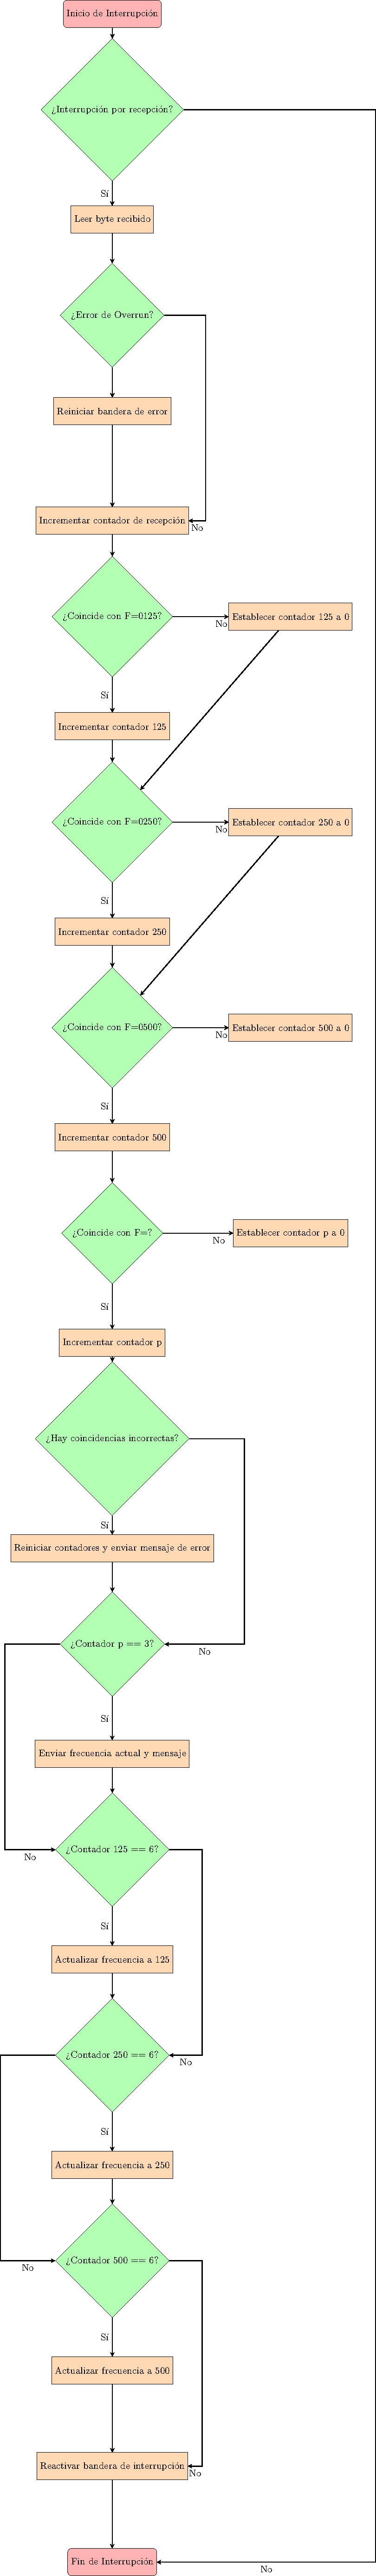
\includepdf{altainterrupcion.pdf}
\subsection{Comunicacion}
\begin{tikzpicture}[node distance=2.5cm]  

% Nodos para la función tx_232  
\node (start1) [startstop] {Inicio tx232};  
\node (checkLength) [decision, below of=start1] {¿longitud > 0?};  
\node (sendChar) [process, below of=checkLength, yshift=-0.5cm] {TXREG1 = *mens};  
\node (clearFlag) [process, below of=sendChar] {PIR1bits.TXIF = 0};  
\node (waitForSend) [process, below of=clearFlag] {Esperar a que TXIF = 1};  
\node (decrement) [process, below of=waitForSend] {longitud-- \\ mens++};  
\node (end1) [startstop, below of=decrement] {Fin tx232};  

% Nodos para la función Envia_cadena  
\node (start2) [startstop, right of=start1, xshift=4cm] {Inicio Enviacadena};  
\node (getLength) [process, below of=start2] {Cantidad = strlen(texto)};  
\node (setBuffer) [process, below of=getLength] {sprintf(buffer, texto)};  
\node (loopBuffer) [process, below of=setBuffer] {For (i=0; i<cantidad)};  
\node (bufferSend) [process, below of=loopBuffer] {TXREG1 = buffer[i]};  
\node (clearFlag2) [process, below of=bufferSend] {PIR1bits.TXIF = 0};  
\node (waitForSend2) [process, below of=clearFlag2] {Esperar a que TXIF = 1};  
\node (end2) [startstop, below of=waitForSend2] {Fin Enviacadena};  

% Nodos para la función Envia_frecuencia  
\node (start3) [startstop, right of=start2, xshift=4cm] {Inicio Enviafrecuencia};  
\node (initVars) [process, below of=start3] {cantdigitos = 0 \\ frecuencia1 = frecval};  
\node (whileLoop) [decision, below of=initVars] {¿frecuencia1 $>$ 0?};  
\node (countDigits) [process, below of=whileLoop, yshift=-0.5cm] {cantdigitos++ \\ frecuencia1 /= 10};  
\node (endWhile) [process, below of=countDigits] {sprintf(buffer, frecval)};  
\node (loopBuffer2) [process, below of=endWhile] {For (i=0; i<cantdigitos)};  
\node (bufferSend2) [process, below of=loopBuffer2] {TXREG1 = buffer[i]};  
\node (clearFlag3) [process, below of=bufferSend2] {PIR1bits.TXIF = 0};  
\node (waitForSend3) [process, below of=clearFlag3] {Esperar a que TXIF = 1};  
\node (end3) [startstop, below of=waitForSend3] {Fin Enviafrecuencia};  

% Conexiones para tx_232  
\draw [arrow] (start1) -- (checkLength);  
\draw [arrow] (checkLength) -- node[anchor=east]{Sí} (sendChar);  
\draw [arrow] (sendChar) -- (clearFlag);  
\draw [arrow] (clearFlag) -- (waitForSend);  
\draw [arrow] (waitForSend) -- (decrement);  
\draw [arrow] (decrement.east) --++ (1,0) --++(0,-2.5) -- node[anchor=south]{No} (end1.east);  
\draw [arrow] (checkLength.west) --++ (-1,0) --++(0,-13) -- node[anchor=south]{No} (end1.west);  

% Conexiones para Envia_cadena  
\draw [arrow] (start2) -- (getLength);  
\draw [arrow] (getLength) -- (setBuffer);  
\draw [arrow] (setBuffer) -- (loopBuffer);  
\draw [arrow] (loopBuffer) -- (bufferSend);  
\draw [arrow] (bufferSend) -- (clearFlag2);  
\draw [arrow] (clearFlag2) -- (waitForSend2);  
\draw [arrow] (waitForSend2.east) --++ (1,0) --++(0,-2.5) -- node[anchor=south]{No} (end2.east);  

% Conexiones para Envia_frecuencia  
\draw [arrow] (start3) -- (initVars);  
\draw [arrow] (initVars) -- (whileLoop);  
\draw [arrow] (whileLoop) -- node[anchor=east]{Sí} (countDigits);  
\draw [arrow] (countDigits) -- (whileLoop);  
\draw [arrow] (whileLoop.east) --++ (1.2,0) --++(0,-5.5) -- node[anchor=south]{No} (endWhile.east);  
\draw [arrow] (endWhile) -- (loopBuffer2);  
\draw [arrow] (loopBuffer2) -- (bufferSend2);  
\draw [arrow] (bufferSend2) -- (clearFlag3);  
\draw [arrow] (clearFlag3) -- (waitForSend3);  
\draw [arrow] (waitForSend3.east) --++ (1,0) --++(0,-2.5) -- node[anchor=south]{No} (end3.east);  

\end{tikzpicture} 